\chapter{Theory}
\label{ch:theory}
\section{Automatic differentiation}
\label{sec:AD}
Automatic differentiation (AD) is a method that makes the computer derive the derivatives with very little effort from the user. If you have not heard of AD before, the first thing that you might think of is algebraic or symbolic differentiation. In this type of differentiation the computer learns the basic rules from calculus like e.g.
\begin{align*}
    &\frac{d}{dx}x^n     = n\cdot x^{n-1} \\
    &\frac{d}{dx}cos(x)  = -sin(x) \\
    &\frac{d}{dx}\exp{x} = \exp{x} \\
\end{align*}
etc. and the chain- and product rule
\begin{align*}
    &\frac{d}{dx}f(x)\cdot g(x) = f'(x)\cdot g(x) + f(x)\cdot g'(x) \\
    &\frac{d}{dx}f(g(x)) = g'(x)\cdot f'(g(x)).
\end{align*}
The computer will then use these rules on symbolic variables to obtain the derivative of any function given. This will give perfectly accurate derivatives, but the disadvantage with this approach is that it is computational demanding and as f(x) becomes more complex, the calculations will become slow.

If AD is not symbolic differentiation you might think that it is finite differences, where you use the definition of the derivative
\begin{equation*}
    \frac{df}{dx} = \frac{f(x+h) - f(x)}{h}
\end{equation*}
with a small h to obtain the numerical approximation of the derivative of f. This approach is not optimal because, first of all, if you choose an h too small, you will get problems with rounding errors on your computer. This is because when h is small, you will subtract two very similar numbers, f(x+h) and f(x) and then divide by a small number h. This means that any small rounding errors in the subtraction will be hugely magnified by the division. Secondly, if you choose h too large your approximation of the derivative will not be accurate. 

AD can be split into two different methods - forward AD and backward AD. Both methods are similar to symbolic differentiation in the way that we implement the differentiation rules, but they differ by instead of differentiating symbols and then inserting values for the symbols, we keep track of the function values and the corresponding values of the derivatives as we go. Both methods does this by separating each expression into a finite set of elementary operations. 

\subsection{Forward Automatic Differentiation}
In forward AD, the function value is stored in a tuple $[\cdot, \cdot]$. In this way, we can continuously update both the function value and the derivative value for every operation we perform on the function. 

As an example, consider the function $f = f(x)$ with its derivative $f_x$ where $x$ is a scalar variable. Then the AD-variable $x$ is the pair $[x, 1]$ and for f we have [$f$, $f_x$]. In the pair $[x,1]$, $x$ is the numerical value of $x$ and $1 = \frac{dx}{dx}$. Similar for $f(x)$ where $f$ is the numerical value of $f(x)$ and $f_x$ the numerical value of $f'(x)$.  We then define the arithmetic operators for such pairs such that for functions $f$ and $g$,
\begin{equation}
    \begin{aligned}
    &\big[f \hspace{0.5em} , \hspace{0.5em}  f_x\big] \pm \big[g \hspace{0.5em} , \hspace{0.5em}  g_x\big] = \big[f \pm g \hspace{0.5em} , \hspace{0.5em}  f_x \pm g_x\big] \hspace{0.5em}, \\\\
    &\big[f \hspace{0.5em} , \hspace{0.5em}  f_x\big]\cdot \big[g \hspace{0.5em} , \hspace{0.5em}  g_x\big] = \big[f\cdot g \hspace{0.5em} , \hspace{0.5em}  f_x\cdot g + f\cdot g_x\big],\\\\
    &\frac{\big[f \hspace{0.5em} , \hspace{0.5em}  f_x\big]}{\big[g \hspace{0.5em} , \hspace{0.5em}  g_x\big]} = \Bigg[\frac{f}{g} \hspace{0.5em} , \hspace{0.5em}  \frac{f_x\cdot g - f\cdot g_x}{g^2}\Bigg].
\end{aligned}
\label{eq:arithmeticOperators}
\end{equation}

It is also necessary to define the chain rule such that for a function h(x)
\begin{equation*}
h\big(f(x)\big) = h\bigg(\big[f \hspace{0.5em} , \hspace{0.5em} f_x\big]\bigg) = \big[h(f) \hspace{0.5em} , \hspace{0.5em}  f_x\cdot h'(f)\big]. 
\end{equation*}
The only thing that remains to define are the rules concerning elementary functions like
\begin{equation}
    \begin{aligned}
    &\exp\bigg(\big[f \hspace{0.5em} , \hspace{0.5em}  f_x\big]\bigg) =  \big[\exp(f) \hspace{0.5em} , \hspace{0.5em}  \exp(f)\cdot f_x\big],\\
    &\log\bigg(\big[f \hspace{0.5em} , \hspace{0.5em}  f_x\big]\bigg) =  \Big[\log(f) \hspace{0.5em} , \hspace{0.5em}  \frac{f_x}{f}\Big],\\
    &\sin\bigg(\big[f \hspace{0.5em} , \hspace{0.5em}  f_x\big]\bigg) =  \big[\sin(f) \hspace{0.5em} , \hspace{0.5em}  \sin(f)\cdot f_x\big]\text{,  etc.}\\
\end{aligned}
\label{eq:elementaryFunctions}
\end{equation}

When these arithmetic operators and the elementary function are implemented you are able to calculate any scalar function derivative without actually doing any form of differentiation yourselves. Let us look at an step by step example where 
\begin{equation}
    \label{eq:forwardADExample}
    f(x) = x\cdot\exp(2x) \hspace{3em} \text{for}\hspace{1em} x = 2.
\end{equation}
Then the declaration of the AD-variable x gives $x = [2 \hspace{0.5em} , \hspace{0.5em}  1]$. All scalars can be looked at as AD variables with derivative equal to 0 such that
\begin{align*}
    2x &= [2 \hspace{0.5em} , \hspace{0.5em}  0]\cdot [2 \hspace{0.5em} , \hspace{0.5em} 1] \\
    &=[2\cdot2 \hspace{0.5em} , \hspace{0.5em}  0\cdot1 + 2\cdot 1]\\
    &=[4 \hspace{0.5em} , \hspace{0.5em} 2].
\end{align*}
After this computation we get from the exponential
\begin{align*}
    \exp(2x) &= \exp\big([4 \hspace{0.5em} , \hspace{0.5em} 2]\big)\\
    &= [\exp(4) \hspace{0.5em} , \hspace{0.5em} \exp(4)\cdot 2],
\end{align*}
and lastly from the product rule we get the correct tuple for $f(x)$
\begin{align*}
    x\cdot \exp(2x) &= [2 \hspace{0.5em} , \hspace{0.5em}  1]\cdot [\exp(4)\hspace{0.5em}, \hspace{0.5em} 2\cdot\exp(4)]\\
    &=[2\cdot\exp(4) \hspace{0.5em} , \hspace{0.5em}  1\cdot \exp(4) + 2\cdot 2\dcot\exp(4)]\\
    [f\hspace{0.5em},\hspace{0.5em} f_x]&=[2\cdot\exp(4) \hspace{0.5em} , \hspace{0.5em} 5\cdot\exp(4)].
\end{align*}
This result is equal
\begin{equation*}
    \big(f(x) \hspace{0.5em},\hspace{0.5em} f_x(x)\big) = \big(x\cdot\exp(2x) \hspace{0.5em},\hspace{0.5em} (1+2x)\exp(2x)\big)
\end{equation*}
for $x = 2$.


\subsection{Dual Numbers}
One approach to implementing forward AD is by dual numbers. Similar to complex numbers dual numbers are defined as 
\begin{equation}
    a + b\epsilon.
    \label{eq:DualNumbers}
\end{equation}
Here $a$ and $b$ are scalars and corresponds to the function value and the derivative value. $\epsilon$ is like we have for complex numbers $i^2 = -1$, but the corresponding relation for dual numbers are $\epsilon^2 = 0$. The convenient part of implementing forward AD with dual numbers is that you get the differentiation rules for arithmetic operations for free. Consider the dual numbers $x$ and $y$ on the form of definition \eqref{eq:DualNumbers}. Then we get for addition
\begin{align*}
x+y &= (a+b\epsilon)+(c+d\epsilon)\\
    &= a+c+(b+d)\epsilon,
\end{align*}
for multiplication
\begin{align*}
x\cdot y &= (a+b\epsilon)\cdot(c+d\epsilon)\\
    &= ac + (ad + bc)\epsilon + bd\epsilon^2 \\
    &= ac + (ad + bc)\epsilon,
\end{align*}
and for division
\begin{align*}
\frac{x}{y} &= \frac{a+b\epsilon}{c+d\epsilon}\\
    &=\frac{a+b\epsilon}{c+d\epsilon} \cdot \frac{c-d\epsilon}{c-d\epsilon}\\
    &=\frac{ac-(ad-bc)\epsilon-bd\epsilon^2}{c^2-d\epsilon^2}\\
    &=\frac{a}{c} + \frac{bc-ad}{c^2}\epsilon.
\end{align*}
This is very convenient, but how does dual numbers handle elementary functions like $\sin$, $\exp$, $\log$ etc? If we look at the Taylor expansion of a function $f(x)$ where x is a dual number, we get
\begin{align*}
    f(x) = f(a+b\epsilon) &= f(a) + \frac{f'(a)}{1!}(b\epsilon) + \frac{f''(a)}{2!}(b\epsilon)^2+...\\
        &=f(a) + f'(a)b\epsilon.
\end{align*}
This means that to make dual numbers handle elementary functions, the first order Taylor expansion needs to be implemented. This equals the implementation of elementary differentiation rules described in equations \eqref{eq:elementaryFunctions}. 

The weakness of implementing AD with dual numbers is clear for functions with multiple variables. Let the function $f$ be defined as $f(x,y,z) = x\cdot y + z$. Let us say we want to know the function value for $(x,y,z) = (2,3,4)$ together with all the derivatives of $f$. First we evaluate $f$ with $x$ as the only varying parameter and the rest as constants:
\begin{align*}
    f(x,y,z) &= (2+1\epsilon)\cdot(3+0\epsilon) + (1+0\epsilon)\\
        &=7+3\epsilon.
\end{align*}
$7$ is now the function value of f, while 3 is the derivative value of f with respect to x, $f_x$. To obtain $f_y$ and $f_z$ we need two more function evaluations with respectively $y$ and $z$ as the varying parameters. This example illustrates the weakness of forward AD implemented with dual numbers - when the function evaluated have many input variables, we need equally many function evaluations to determine the jacobian of the function.

\subsection{Backward Automatic Differentiation}
The main disadvantage with forward AD is when there are many input variables and you want the derivative with respect to all variables. This is where Backward AD is a more efficient way of obtaining the derivatives. To explain backward AD it is easier to first consider the approach for forward AD, where the method also can be be explained as an extensive use of the chain rule
\begin{equation}
    \label{eq:chainRule}
    \frac{\partial f}{\partial t} = \sum_i\left(\frac{\partial f}{\partial g_i}\cdot\frac{\partial g_i}{\partial t}\right).
\end{equation}
Take $f(x) = x\cdot\exp(2x)$ like in the forward AD example \eqref{eq:forwardADExample}. We then split up the function into a sequence of elementary functions
\begin{equation}
    \label{eq:BackwardADSeperationSimple}
    x, \hspace{2em} g_1 = 2x, \hspace{2em} g_2 = \exp(g_1), \hspace{2em} g_3 = x\cdot g_2,
\end{equation}
where clearly $f(x) = g_3$. If we want the derivative of $f$ with respect to $x$ we can obtain expressions for all $g$'s by using the chain rule \eqref{eq:chainRule}
\begin{align*}
     \frac{\partial x}{\partial x} &= 1, \\
     \frac{\partial g_1}{\partial x} &= 2, \\
     \frac{\partial g_2}{\partial x} &= \frac{\partial}{\partial g_1}\exp(g_1)\cdot\frac{\partial g_1}{\partial x} = 2\exp(2x).
\end{align*}
Lastly by calculating the derivative of $g_3$ with respect to $x$ in the same matter yields the expression for the derivative of f
\begin{align*}
    \frac{\partial f}{\partial x} &= \frac{\partial g_3}{\partial x}\\
    &=\frac{\partial x}{\partial x}\cdot g_2 + x\cdot\frac{\partial g_2}{\partial x}\\
    &= \exp(2x) + x\cdot 2\exp(2x) \\
    &= (1+2x)\exp(2x).
\end{align*}
This shows how forward AD actually uses the chain rule on a sequence of elementary functions with respect to the independent variables, in this case $x$. Backward AD also uses the chain rule, but in the opposite direction. It uses it with respect to dependent variables. The chain rule then has the form
\begin{equation}
    \label{eq:chainRuleReverse}
    \frac{\partial s}{\partial u} = \sum_i\left(\frac{\partial f_i}{\partial u}\cdot\frac{\partial s}{\partial f_i}\right),
\end{equation}
for some s to be chosen. The same example with $f(x) = x\cdot\exp(2x)$ and with the same sequence of elementary functions like in \eqref{eq:BackwardADSeperationSimple} gives the expressions from the chain rule \eqref{eq:chainRuleReverse}
\begin{align*}
    \frac{\partial s}{\partial g_3} &= \text{Unknown}\\
    \frac{\partial s}{\partial g_2} &= \frac{\partial g_3}{\partial g_2} \cdot \frac{\partial s}{\partial g_3} &&\Longleftrightarrow \quad x\cdot \frac{\partial s}{\partial g_3} \\
    \frac{\partial s}{\partial g_1} &= \frac{\partial g_2}{\partial g_1}\cdot \frac{\partial s}{\partial g_2} &&\Longleftrightarrow \quad g_2 \cdot \frac{\partial s}{\partial g_2} \\
    \frac{\partial s}{\partial x} &= \frac{\partial g_3}{\partial x}\cdot \frac{\partial s}{\partial g_3} + \frac{\partial g_1}{\partial x}\cdot \frac{\partial s}{\partial g_1} && \Longleftrightarrow \quad g_2\cdot \frac{\partial s}{\partial g_3} + 2\cdot \frac{\partial s}{\partial g_1}.\\
\end{align*}
By substituting $s$ with $g_3$ gives
\begin{align*}
    \frac{\partial g_3}{\partial g_3} &= 1\\
    \frac{\partial g_3}{\partial g_2} &= x\\
    \frac{\partial g_3}{\partial g_1} &= \exp(2x)\cdot x\\
    \frac{\partial g_3}{\partial x} &= \exp(2x)\cdot 1 + 2\cdot\exp(2x)\cdot x = (1 + 2x)\exp(2x),\\
\end{align*}
hence we obtain the correct derivative $f_x$. By now you might wonder why make this much effort to obtain the derivative of f compared to just using forward AD. The answer to this comes by looking at a more complex function with multiple input parameters. Let $f(x,y,z) = z(\sin(x^2)+yx)$ and 
\begin{equation*}
    g_1 = x^2, \quad g_2 = x\cdot y, \quad g_3 = \sin(g_1), \quad g_4 = g_2 + g_3, \quad g_5 = z\cdot g_4.
\end{equation*}
Now the derivatives from the chain rule in equation \eqref{eq:chainRuleReverse} becomes \\
\begin{multicols}{3}
    \noindent
    \begin{align*}
        \frac{\partial s}{\partial g_5} &= \text{Unknown}\\
        \frac{\partial s}{\partial g_4} &= z\cdot\frac{\partial s}{\partial g_5}\\
        \frac{\partial s}{\partial g_3} &= \frac{\partial s}{\partial g_4}
    \end{align*}
    \begin{align*}
        \frac{\partial s}{\partial g_2} &= \frac{\partial s}{\partial g_4} \\
        \frac{\partial s}{\partial g_1} &= \cos(g_1)\frac{\partial s}{\partial g_3}\\
        \frac{\partial s}{\partial x}   &= 2x\cdot\frac{\partial s}{\partial g_1} + y\cdot\frac{\partial s}{\partial g_2}
    \end{align*}
    \begin{align*}
        \frac{\partial s}{\partial y}   &= x\cdot\frac{\partial s}{\partial g_2}\\
        \frac{\partial s}{\partial z}   &= g_4\cdot\frac{\partial s}{\partial g_5}
    \end{align*}
\end{multicols}

substituting $s$ with $g_5$ yields
\begin{multicols}{3}
    \noindent
    \begin{align*}
        \frac{\partial g_5}{\partial g_5} &= 1\\
        \frac{\partial g_5}{\partial g_4} &= z\\
        \frac{\partial g_5}{\partial g_3} &= z
    \end{align*}
    \begin{align*}
        \frac{\partial g_5}{\partial g_2} &= z\\
        \frac{\partial g_5}{\partial g_1} &= \cos(x^2)\cdot z\\
        \frac{\partial g_5}{\partial x}   &= 2x\cdot\cos(x^2)\cdot z + yz
    \end{align*}
    \begin{align*}
        \frac{\partial g_5}{\partial y}   &= xz\\
        \frac{\partial g_5}{\partial z}   &= \sin(x^2)+xy
    \end{align*}
\end{multicols}
The calculation of the derivatives together with a dependency graph can be seen in figure \ref{fig:depency_graph_backward_AD}. This shows that we get all the derivatives of $f(x) = g_5$ with a single function evaluation!
\begin{figure}[htbp]
	\centering
	    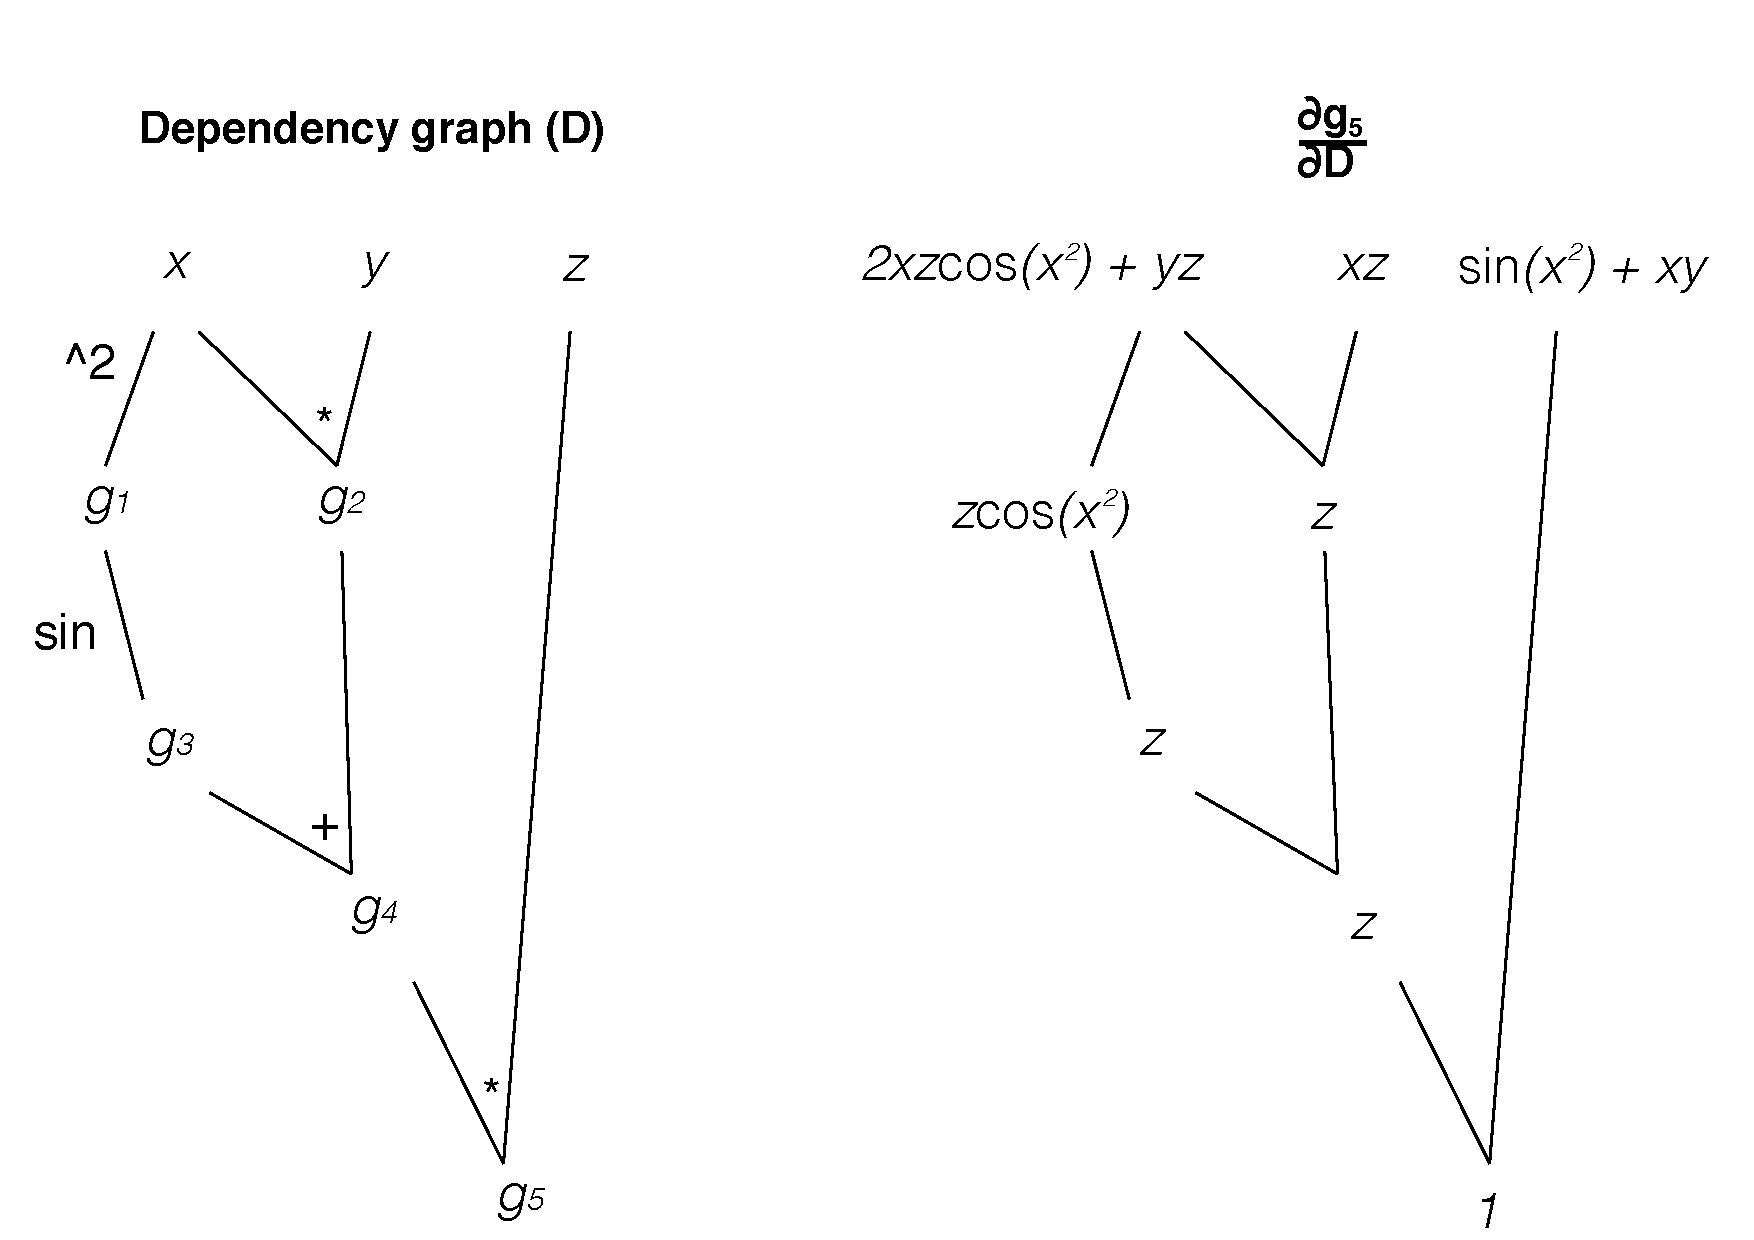
\includegraphics[width=0.9\textwidth]{figures/dependency_graph_backward_AD.pdf}
	    \caption{NOT A FINISHED FIGURE. Just a quick sketch of the idea I have of visualising the process of backward AD as i felt it got a bit messy with all the expressions. Gladly receiving comments on the thought/suggestions to make it more clear}
	\label{fig:depency_graph_backward_AD}
\end{figure}
Comparing this to the method of Dual Numbers were we would have to evaluate $f$ three times, one for each derivative, this is a big improvement. This illustrates the strength of backward AD - no matter how many input parameters a function have, you only need one function evaluation to get all the derivatives of a function. The disadvantage of backward AD is that, in differ from what we did in the example above when we did it by hand, we still only want to carry along the function value and the derivative value as we did in forward AD. This means that we have to implement the dependency tree shown in figure \ref{fig:depency_graph_backward_AD}. This makes the implementation of backward AD much harder than for forward AD and a bad implementation of this tree will reduce the advantage of backward AD. This is the reason why we here will have focus on implementing forward AD.

\subsection{Forward Automatic Differentiation with multiple parameters}
\textbf{TODO: Endre under så dette glir inn med det som er skrevet om BackwardAD over}
To handle the problem of many function evaluations in forward AD when having a function with many input parameters one can look at the method described by Knut-Andreas Lie in \emph{\citet{lieMrstUrl}}. Say we have three variables x, y and z. Then the corresponding AD-variables becomes
\begin{equation*}
    [x\hspace{0.5em},\hspace{0.5em}(1,0,0)^\top]\hspace{2em},\hspace{2em}
    [y\hspace{0.5em},\hspace{0.5em}(0,1,0)^\top]\hspace{2em},\hspace{2em}
    [z\hspace{0.5em},\hspace{0.5em}(0,0,1)^\top].
\end{equation*}

There are now not only one scalar as the derivative value, but the gradient to the corresponding variable. The operators defined in Equations \ref{eq:arithmeticOperators} and the elementary functions in Equations \ref{eq:elementaryFunctions} are still valid, but instead of scalar products there are now vector products. As an example let $f(x,y,z) = xyz$ and $x = 1$, $y = 2$ and $z = 3$, then
\begin{align*}
    xyz &= [1\hspace{0.5em},\hspace{0.5em}(1,0,0)^\top]\cdot [2\hspace{0.5em},\hspace{0.5em}(0,1,0)^\top]\cdot
    [3\hspace{0.5em},\hspace{0.5em}(0,0,1)^\top] \\
    &=[1\cdot 2\cdot 3\hspace{0.5em},\hspace{0.5em}2\cdot3\cdot(1,0,0)^\top + 1\cdot3\cdot(0,1,0)^\top + 1\cdot2\cdot(0,0,1)^\top] \\
    [f\hspace{0.5em},\hspace{0.5em}f_x] &= [6\hspace{0.5em},\hspace{0.5em}(6,3,2)^\top].
\end{align*}
This result is equal to the tuple
\begin{equation*}
    \big(f(x,y,z) \hspace{0.5em},\hspace{0.5em} \nabla f(x,y,z)\big) = \big(xyz \hspace{0.5em},\hspace{0.5em} (yz,xz,xy)^\top\big)
\end{equation*}
for the corresponding $x$, $y$ and $z$ values. \\


\section{Julia}

















